\documentclass[12pt]{article}
\usepackage{graphicx}
\usepackage{caption}
\usepackage[hypcap=false]{caption}
\usepackage{geometry}
\usepackage{listings}
\usepackage{amsthm}
\geometry{margin=1in}
\RequirePackage{amsmath}
\usepackage{cite}
\usepackage{booktabs}
\usepackage{amsmath,amssymb,amsfonts,amsthm}
\usepackage{algorithmic}
\usepackage{textcomp}
\usepackage{xcolor}
\usepackage{txfonts}
\usepackage{enumitem}
\usepackage{mathtools}
\usepackage{gensymb}
\usepackage{comment}
\usepackage[breaklinks=true]{hyperref}
\usepackage{tkz-euclide} 
\usepackage{listings}                                                            \usepackage[utf8]{inputenc}     
\usepackage{xparse}
\usepackage{color}                                            
\usepackage{array}                                            
\usepackage{longtable}                                       
\usepackage{calc}               
\usepackage{multirow}
\usepackage{multicol}
\usepackage[version=4]{mhchem} 
\usepackage{hhline}                                           
\usepackage{ifthen}                                           
\usepackage{lscape}
\usepackage{tabularx}
\usepackage{array}
\usepackage{float}
\usepackage{gvv}
\usepackage{gvv-book}


\author{EE25BTECH11010-ARSH DHOKE}
\title{GATE CY 2020 questions}
\date{}

\begin{document}
\maketitle

\section*{GA - General Aptitude}
\textbf{Q1 - Q5 carry one mark each.}

\begin{enumerate}
\item While I agree \underline{\hspace{2cm}} his proposal this time, I do not often agree \underline{\hspace{2cm}} him.
\begin{multicols}{2}
\begin{enumerate}
\item to, with
\item with, to
\item with, with
\item to, to
\end{enumerate}
\end{multicols}
\hfill (GATE CY 2020)

\item The recent measures to improve the output would \underline{\hspace{2cm}} the level of production to our satisfaction.
\begin{multicols}{2}
\begin{enumerate}
\item increase
\item decrease
\item speed
\item equalise
\end{enumerate}
\end{multicols}
\hfill (GATE CY 2020)

\item Select the word that fits the analogy:

White: Whitening :: Light: \underline{\hspace{2cm}}
\begin{enumerate}
\begin{multicols}{2}
\item Lightning
\item Lightening
\item Lighting
\item Enlightening
\end{multicols}
\end{enumerate}
\hfill (GATE CY 2020)


\item In one of the greatest innings ever seen in 142 years of Test history, Ben Stokes upped the tempo in a five-and-a-half hour long stay of 219 balls including 11 fours and 8 sixes that saw him finish on 135 not out as England squared the five-match series.

Based on their connotations in the given passage, which one of the following meanings DOES NOT match?
\begin{enumerate}
\begin{multicols}{2}
\item upped = increased
\item squared = lost
\item tempo = enthusiasm
\item saw = resulted in
\end{multicols}
\end{enumerate}
\hfill (GATE CY 2020)

\item There are five levels \{P, Q, R, S, T\} in a linear supply chain before a product reaches customers, as shown in the figure.
\begin{figure}[H]
    \centering
    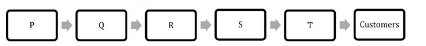
\includegraphics[width=0.4\columnwidth]{figs/q5.png}
    \caption{Figure for Q.5}
    \label{fig:q5}
\end{figure}
At each of the five levels, the price of the product is increased by 25\%. If the product is produced at level P at the cost of Rs. 120 per unit, what is the price paid (in rupees) by the customers?
\begin{multicols}{2}
\begin{enumerate}
\item 187.50
\item 234.38
\item 292.96
\item 366.21
\end{enumerate}
\end{multicols}
\hfill (GATE CY 2020)

\textbf{Q6 - Q10 carry two marks each.}


\item Climate change and resilience deal with two aspects – reduction of sources of non-renewable energy resources and reducing vulnerability of climate change aspects. The terms ‘mitigation’ and ‘adaptation’ are used to refer to these aspects, respectively.

Which of the following assertions is best supported by the above information?
\begin{enumerate}
\item Mitigation deals with consequences of climate change.
\item Adaptation deals with causes of climate change.
\item Mitigation deals with actions taken to reduce the use of fossil fuels.
\item Adaptation deals with actions taken to combat green-house gas emissions.
\end{enumerate}
\hfill (GATE CY 2020)

\item Find the missing element in the following figure.

\begin{figure}[H]
\centering
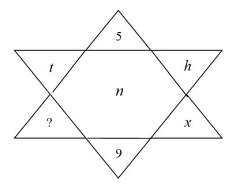
\includegraphics[width=0.4\columnwidth]{figs/q7.png}
\caption{Figure for Q.7}
\label{fig:q7}
\end{figure}
\begin{enumerate}
\begin{multicols}{2}
\item $d$
\item $e$
\item $w$
\item $y$
\end{multicols}
\end{enumerate}
\hfill (GATE CY 2020)

\item It was estimated that 52 men can complete a strip in a newly constructed highway connecting cities P and Q in 10 days. Due to an emergency, 12 men were sent to another project. How many number of days, more than the original estimate, will be required to complete the strip?
\begin{enumerate}
\begin{multicols}{2}
\item 3 days
\item 5 days
\item 10 days
\item 13 days
\end{multicols}
\end{enumerate}
\hfill (GATE CY 2020)

\item An engineer measures THREE quantities $X$, $Y$ and $Z$ in an experiment. She finds that they follow a relationship that is represented in the figure below: (the product of $X$ and $Y$ linearly varies with $Z$)

\begin{figure}[H]
\centering
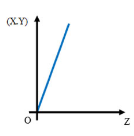
\includegraphics[width=0.4\columnwidth]{figs/q9.png}
\caption{Figure for Q.9}
\label{fig:q9}
\end{figure}

Then, which of the following statements is FALSE?
\begin{enumerate}
\item For fixed $Z$, $X$ is proportional to $Y$
\item For fixed $Y$, $X$ is proportional to $Z$
\item For fixed $X$, $Z$ is proportional to $Y$
\item $XY/Z$ is constant
\end{enumerate}
\hfill (GATE CY 2020)

\item The two pie-charts given below show the data of total students and only girls registered in different streams in a university. If the total number of students registered in the university is $5000$, and the total number of registered girls is $1500$, then, the ratio of boys enrolled in Arts to the girls enrolled in Management is \underline{\hspace{1cm}}.

\begin{figure}[H]
\centering
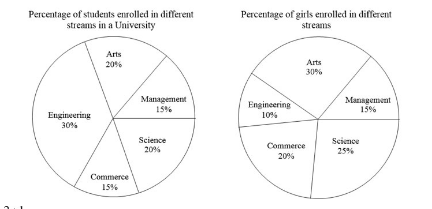
\includegraphics[width=0.6\columnwidth]{figs/q10.png}
\caption{Figure for Q.10}
\label{fig:q10}
\end{figure}

\begin{enumerate}
\begin{multicols}{2}
\item $2 : 1$
\item $9 : 22$
\item $11 : 9$
\item $22 : 9$
\end{multicols}
\end{enumerate}
\hfill (GATE CY 2020)


\section*{CY: Chemistry}
\textbf{Q1 - Q25 carry one mark each.}

\setcounter{enumi}{0}

\item Among the following, the suitable reagents for the given transformation is:

\begin{figure}[H]
    \centering
    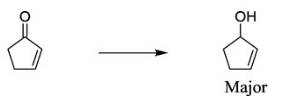
\includegraphics[width=0.4\columnwidth]{figs/q1.png}
    \caption{Figure for Q.1}
    \label{fig:q1}
\end{figure}

\begin{enumerate}
\begin{multicols}{2}
\item H$_2$, Pd / C
\item H$_2$N--NH$_2$ / KOH, $\Delta$
\item NaBH$_4$ / CeCl$_3\cdot$7H$_2$O
\item Li / Liq. NH$_3$
\end{multicols}
\end{enumerate}
\hfill (GATE CY 2020)

\item Major product formed in the following reaction sequence is:

\begin{figure}[H]
    \centering
    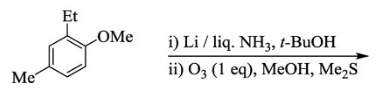
\includegraphics[width=0.4\columnwidth]{figs/q2.png}
    \caption{Figure for Q.2}
    \label{fig:q2}
\end{figure}


\begin{enumerate}
\item
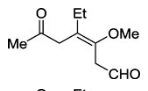
\includegraphics[width=0.4\columnwidth]{figs/q2a.png}
\captionof{figure}{Option A}
\label{fig:q2a}
\item
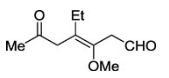
\includegraphics[width=0.4\columnwidth]{figs/q2b.png}
\captionof{figure}{Option B}
\label{fig:q2b}
\item
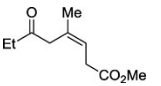
\includegraphics[width=0.4\columnwidth]{figs/q2c.png}
\captionof{figure}{Option C}
\label{fig:q2c}
\item
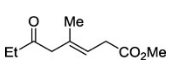
\includegraphics[width=0.4\columnwidth]{figs/q2d.png}
\captionof{figure}{Option D}
\label{fig:q2d}
\end{enumerate}
\hfill (GATE CY 2020)

    \item Major product formed in the following reaction is:
    
    \begin{center}
        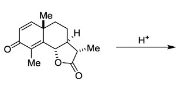
\includegraphics[width=0.6\columnwidth]{figs/q3.png}
        \captionof{figure}{Figure for Q.3}
\label{fig:q3}
    \end{center}

    \begin{enumerate}
        \item 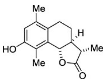
\includegraphics[width=0.4\columnwidth]{figs/q3a.png}
        \captionof{figure}{Option A}
\label{fig:q3a}
        \item 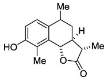
\includegraphics[width=0.4\columnwidth]{figs/q3b.png}
        \captionof{figure}{Option B}
\label{fig:q3b}
        \item 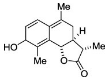
\includegraphics[width=0.4\columnwidth]{figs/q3c.png}
        \captionof{figure}{Option C}
\label{fig:q3c}
        \item 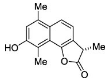
\includegraphics[width=0.4\columnwidth]{figs/q3d.png}
        \captionof{figure}{Option D}
\label{fig:q3d}
    \end{enumerate}
    \hfill (GATE CY 2020)

    \item Major product formed in the following transformation is:
    
    \begin{center}
        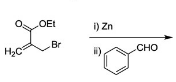
\includegraphics[width=0.6\columnwidth]{figs/q4.png}
         \captionof{figure}{Figure for Q.4}
\label{fig:q4}
    \end{center}

    \begin{enumerate}
        \item 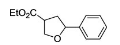
\includegraphics[width=0.4\columnwidth]{figs/q4a.png}
        \captionof{figure}{Option A}
\label{fig:q4a}
        \item 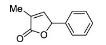
\includegraphics[width=0.4\columnwidth]{figs/q4b.png}
        \captionof{figure}{Option B}
\label{fig:q4b}
        \item 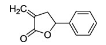
\includegraphics[width=0.4\columnwidth]{figs/q4c.png}
        \captionof{figure}{Option C}
\label{fig:q4c}
        \item 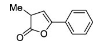
\includegraphics[width=0.4\columnwidth]{figs/q4d.png}
        \captionof{figure}{Option D}
\label{fig:q4d}
    \end{enumerate}
    \hfill (GATE CY 2020)

\item Absolute stereochemistry of the given compound is:

\begin{center}
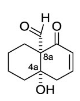
\includegraphics[width=0.4\columnwidth]{figs/Q5.png}
 \captionof{figure}{Figure for Q.5}
\label{fig:Q5}
\end{center}

\begin{enumerate}
\begin{multicols}{2}
    \item 4aR, 8aS
    \item 4aR, 8aR
    \item 4aS, 8aS
    \item 4aS, 8aR
    \end{multicols}
\end{enumerate}
\hfill (GATE CY 2020)

\item In the following reaction sequence:

\begin{center}
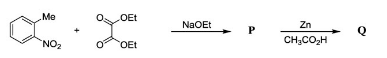
\includegraphics[width=\columnwidth]{figs/q6.png}
 \captionof{figure}{Figure for Q.6}
\label{fig:q6}
\end{center}

The major products P and Q are:

\begin{enumerate}
    \item 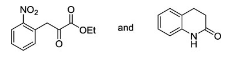
\includegraphics[width=0.4\columnwidth]{figs/q6a.png}
    \captionof{figure}{Option A}
\label{fig:q6a}
    \item 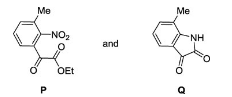
\includegraphics[width=0.4\columnwidth]{figs/q6b.png}
    \captionof{figure}{Option B}
\label{fig:q6b}
    \item 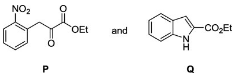
\includegraphics[width=0.4\columnwidth]{figs/q6c.png}
    \captionof{figure}{Option C}
\label{fig:q6c}
    \item 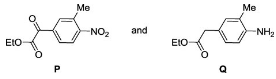
\includegraphics[width=0.4\columnwidth]{figs/q6d.png}
    \captionof{figure}{Option D}
\label{fig:q6d}
\end{enumerate}
\hfill (GATE CY 2020)

\item Major product formed in the given reaction is:

\begin{center}
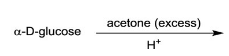
\includegraphics[width=0.4\columnwidth]{figs/Q7.png}
 \captionof{figure}{Figure for Q.7}
\label{fig:Q7}
\end{center}

\begin{enumerate}
    \item 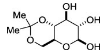
\includegraphics[width=0.4\columnwidth]{figs/q7a.png}
    \captionof{figure}{Option A}
\label{fig:q7a}
    \item 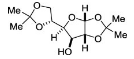
\includegraphics[width=0.4\columnwidth]{figs/q7b.png}
    \captionof{figure}{Option B}
\label{fig:q7b}
    \item 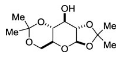
\includegraphics[width=0.4\columnwidth]{figs/q7c.png}
    \captionof{figure}{Option C}
\label{fig:q7c}
    \item 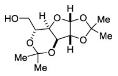
\includegraphics[width=0.4\columnwidth]{figs/q7d.png}
    \captionof{figure}{Option D}
\label{fig:q7d}
\end{enumerate}
\hfill (GATE CY 2020)

\item The \textbf{CORRECT} statement regarding the substitution of coordinated ligands in Ni(CO)$_4$ and Co(NO)(CO)$_3$ is:

\begin{enumerate}
    \item Ni(CO)$_4$ and Co(NO)(CO)$_3$ follow associative and dissociative pathways, respectively.
    \item Ni(CO)$_4$ and Co(NO)(CO)$_3$ follow dissociative and associative pathways, respectively.
    \item Both Ni(CO)$_4$ and Co(NO)(CO)$_3$ follow associative pathway.
    \item Both Ni(CO)$_4$ and Co(NO)(CO)$_3$ follow dissociative pathway.
\end{enumerate}
\hfill (GATE CY 2020)

\item The \textbf{CORRECT} statement about hexagonal boron nitride is:

\begin{enumerate}
    \item It is a good electrical conductor.
    \item It has same layer stacking as that of graphite.
    \item It is reactive towards fluorine.
    \item It has lower thermal stability in air compared to that of graphite.
\end{enumerate}
\hfill (GATE CY 2020)

\item In oxyhemocyanin, the coordination number, mode of oxygen binding, color and the net magnetic behavior of copper ions, respectively are:

(Given: atomic number of Cu is 29)

\begin{enumerate}
    \item Four, $\mu$-$\eta^2:\eta^1$-O$_2^-$, colorless and paramagnetic.
    \item Five, $\mu$-$\eta^2:\eta^2$-O$_2^-$, colorless and paramagnetic.
    \item Five, $\mu$-$\eta^2:\eta^2$-O$_2^-$, blue and diamagnetic.
    \item Four, $\mu$-$\eta^2:\eta^1$-O$_2^-$, blue and diamagnetic.
\end{enumerate}
\hfill (GATE CY 2020)


\item Among the following species, the one that has pentagonal shape is:
(Given: atomic numbers of O, F, S, I and Xe are 8, 9, 16, 53 and 54, respectively.)
\begin{multicols}{2}
\begin{enumerate}
    \item $\mathrm{XeOF_4}$
    \item $\mathrm{IF_5}$
    \item $[\mathrm{SF_6}]^{-}$
    \item $[\mathrm{XeF_5}]^{-}$
\end{enumerate}
\end{multicols}
\hfill (GATE CY 2020)

\item A solution containing a metal complex absorbs at $480\,\mathrm{nm}$ with molar extinction coefficient of $15{,}000\ \mathrm{L\,mol^{-1}\,cm^{-1}}$. If the path length of the cell is $1.0\ \mathrm{cm}$ and transmittance is $20.5\%$, the concentration (in $\mathrm{mol\,L^{-1}}$) of the metal complex is:
\begin{multicols}{2}
\begin{enumerate}
    \item $1.37\times10^{-5}$
    \item $2.29\times10^{-5}$
    \item $4.59\times10^{-5}$
    \item $8.75\times10^{-5}$
\end{enumerate}
\end{multicols}
\hfill (GATE CY 2020)

\item Among the following linear combination of atomic orbitals, the \textbf{CORRECT} representation of the lowest unoccupied $\pi$-molecular orbital of butadiene is:
\begin{multicols}{2}
\begin{enumerate}
    \item $\psi=-0.372\,\phi_1+0.602\,\phi_2-0.602\,\phi_3+0.372\,\phi_4$
    \item $\psi=0.602\,\phi_1-0.372\,\phi_2-0.372\,\phi_3+0.602\,\phi_4$
    \item $\psi=0.602\,\phi_1+0.372\,\phi_2-0.372\,\phi_3-0.602\,\phi_4$
    \item $\psi=0.372\,\phi_1+0.602\,\phi_2+0.602\,\phi_3+0.372\,\phi_4$
\end{enumerate}
\end{multicols}
\hfill (GATE CY 2020)

\item The activity of an $m$ molal CuSO$_4$ solution can be expressed in terms of its mean activity coefficient $\gamma_{\pm}$ as:
\begin{multicols}{2}
\begin{enumerate}
    \item $m^{2}\gamma_{\pm}^{2}$
    \item $4m^{3}\gamma_{\pm}^{3}$
    \item $16m^{4}\gamma_{\pm}^{4}$
    \item $108m^{5}\gamma_{\pm}^{5}$
\end{enumerate}
\end{multicols}
\hfill (GATE CY 2020)

\item The character table for a pyramidal AB$_3$ molecule of C$_{3v}$ point group is given below:

\begin{center}
\begin{center}
\begin{tabular}{ll}
    \textbf{Group I} & \textbf{Group II} \\
    P. Ferrite & 1. Hexagonal Close Packed (HCP) \\
    Q. Austenite & 2. Body Centered Cubic (BCC) \\
    R. Martensite & 3. Body Centered Tetragonal (BCT) \\
    & 4. Face Centered Cubic (FCC)
\end{tabular}
\end{center}
 \captionsetup{type=table}
\captionof{table}{Table 1 for Q.15}
\end{center}

The reducible representation of pyramidal AB$_3$ is:

\begin{center}
\begin{tabular}{|c|c|c|}
     \hline
     \textbf{Mineral} & \textbf{Modal abundance \brak{\%}} & \textbf{Partition coefficient}\\
     \hline
     Clinopyroxene & $45$ & $0.506$ \\
      \hline
      Orthopyroxene & $40$ & $0.42$ \\
      \hline
      Olivine & $10$ & $0.045$ \\
      \hline
      Plagioclase & $05$ & $0.019$ \\
      \hline
\end{tabular}
 \captionsetup{type=table}
\captionof{table}{Table 2 for Q.15}
\end{center}

The \textbf{CORRECT} option representing all the normal Raman active modes of pyramidal AB$_3$ is:

\begin{multicols}{2}
\begin{enumerate}
    \item $A_1 + A_2 + 2E$
    \item $3E$
    \item $3A_1 + A_2 + E$
    \item $2A_1 + 2E$
\end{enumerate}
\end{multicols}
\hfill (GATE CY 2020)

\item In the following reaction:
\begin{figure}[H]
    \centering
    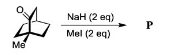
\includegraphics[width=0.4\columnwidth]{figs/q16.png}
    \caption{Figure for Q.16}
    \label{fig:q16}
\end{figure}
the number of peaks exhibited by the major product P in its broadband proton decoupled $^{13}$C NMR spectrum is \underline{\hspace{2cm}}.
\hfill (GATE CY 2020)

\item Among the following:
\begin{figure}[H]
    \centering
    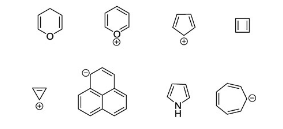
\includegraphics[width=0.4\columnwidth]{figs/q17.png}
    \caption{Figure for Q.17}
    \label{fig:q17}
\end{figure}
the total number of aromatic species is \underline{\hspace{2cm}}.
\hfill (GATE CY 2020)

\item The maximum number of microstates for $d^2$ electronic configuration is \underline{\hspace{2cm}}.


\item In a uranium recovery process, an aqueous solution of uranyl ion is evaporated, dried in air at 400 $^\circ$C and subsequently reduced with hydrogen at 700 $^\circ$C to obtain a uranium compound (X). The oxidation state of uranium in X is \underline{\hspace{2cm}}.

(Given: atomic number of U is 92)
\hfill (GATE CY 2020)

\item For a cubic crystal system, the powder X-ray diffraction pattern recorded using Cu K$_\alpha$ source ($\lambda = 1.54$ \AA) shows a peak at 33.60$^\circ$ for (111) plane. The lattice parameter 'a' (in \AA, \textit{rounded off to two decimal places}) is \underline{\hspace{2cm}}.
\hfill (GATE CY 2020)

\item In an NMR spectrometer operating at a magnetic field strength of 16.45 T, the resonance frequency (in MHz, \textit{rounded off to one decimal place}) of $^{19}$F nucleus is \underline{\hspace{2cm}}.

(Given: g factor of $^{19}$F = 5.255; $\beta_N = 5.05 \times 10^{-27}$ J T$^{-1}$; $h = 6.626 \times 10^{-34}$ J s)
\hfill (GATE CY 2020)

\item When three moles of helium is mixed with one mole of neon at constant temperature and pressure (25 $^\circ$C, 1 atm), the entropy of mixing (in J K$^{-1}$, \textit{rounded off to two decimal places}) is \underline{\hspace{2cm}}.

(Given: R = 8.314 J K$^{-1}$ mol$^{-1}$)
\hfill (GATE CY 2020)

\item At 25 $^\circ$C, the emf (\textit{in volts, rounded off to three decimal places}) of the cell,

Ag $|$ AgBr(s) $|$ Br$^-$ (a = 0.20), Cu$^{2+}$ (a = 0.48), Cu$^+$ (a = 0.24) $|$ Pt is \underline{\hspace{2cm}}.

(Given: The standard emf of the cell is 0.082 V; R = 8.314 J K$^{-1}$ mol$^{-1}$; F = 96500 C mol$^{-1}$)
\hfill (GATE CY 2020)

\item For an enzyme catalyzed reaction, the plot of inverse of initial rate against inverse of initial substrate concentration is linear with slope 0.16 s and intercept 2.12 mol$^{-1}$ L s. The estimated value of Michaelis constant (in mol L$^{-1}$, \textit{rounded off to two decimal places}) is \underline{\hspace{2cm}}.
\hfill (GATE CY 2020)

\item Fluorescence quantum yield and fluorescence lifetime of a molecule are 0.4 and $5 \times 10^{-9}$ s, respectively. If the fluorescence decay rate constant is Y $\times 10^7$ s$^{-1}$, the value of Y (\textit{rounded off to nearest integer}) is \underline{\hspace{2cm}}.
\hfill (GATE CY 2020)


\textbf{Q.26 - Q.55 carry two marks each.}

\item Major product formed in the following reaction sequence is:

\begin{center}
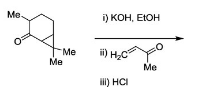
\includegraphics[width=0.6\columnwidth]{figs/q26.png}
 \captionof{figure}{Figure for Q.26}
 \label{fig:q26}
\end{center}

\begin{enumerate}
\item 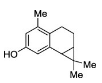
\includegraphics[width=0.25\columnwidth]{figs/q26a.png}
 \captionof{figure}{Option A}
    \label{fig:q26a}
\item 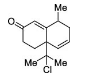
\includegraphics[width=0.25\columnwidth]{figs/q26b.png}
 \captionof{figure}{Option B}
    \label{fig:q26b}
\item 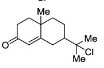
\includegraphics[width=0.25\columnwidth]{figs/q26c.png}
 \captionof{figure}{Option C}
    \label{fig:q26c}
\item 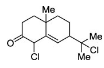
\includegraphics[width=0.25\columnwidth]{figs/q26d.png}
 \captionof{figure}{Option D}
    \label{fig:q26d}
\end{enumerate}
\hfill (GATE CY 2020)

\item Major products \textbf{P} and \textbf{Q}, in the given reaction sequence, are:

\begin{center}
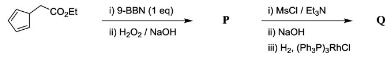
\includegraphics[width=0.6\columnwidth]{figs/q27.png}
\captionof{figure}{Figure for Q.27}
 \label{fig:q27}
\end{center}

\begin{enumerate}
\item 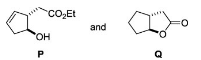
\includegraphics[width=0.4\columnwidth]{figs/q27a.png}
\captionof{figure}{Option A}
    \label{fig:q27a}
\item 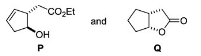
\includegraphics[width=0.4\columnwidth]{figs/q27b.png}
\captionof{figure}{Option B}
    \label{fig:q27b}
\item 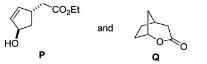
\includegraphics[width=0.4\columnwidth]{figs/q27c.png}
\captionof{figure}{Option C}
    \label{fig:q27c}
\item 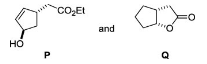
\includegraphics[width=0.4\columnwidth]{figs/q27d.png}
\captionof{figure}{Option D}
    \label{fig:q27d}
\end{enumerate}
\hfill (GATE CY 2020)

\item Major products \textbf{P} and \textbf{Q}, formed in the reactions given below, are:

\begin{center}
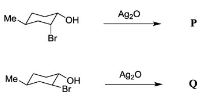
\includegraphics[width=0.6\columnwidth]{figs/q28.png}
\captionof{figure}{Figure for Q.28}
 \label{fig:q28}
\end{center}

\begin{enumerate}
\item 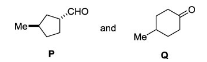
\includegraphics[width=0.4\columnwidth]{figs/q28a.png}
\captionof{figure}{Option A}
    \label{fig:q28a}
\item 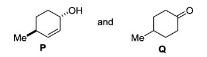
\includegraphics[width=0.4\columnwidth]{figs/q28b.png}
\captionof{figure}{Option B}
    \label{fig:q28b}
\item 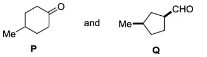
\includegraphics[width=0.4\columnwidth]{figs/q28c.png}
\captionof{figure}{Option C}
    \label{fig:q28c}
\item 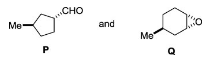
\includegraphics[width=0.4\columnwidth]{figs/q28d.png}
\captionof{figure}{Option D}
    \label{fig:q28d}
\end{enumerate}
\hfill (GATE CY 2020)

\item A compound with molecular formula C$_{10}$H$_{12}$O$_2$ showed a strong IR band at $\sim$ 1720 cm$^{-1}$, a peak at m/z 122 in the mass spectrum and the following $^1$H NMR signals: $\delta$ 8.1--8.0 (2H, m), 7.6--7.5 (1H, m), 7.5--7.3 (2H, m), 4.3 (2H, t), 1.8 (2H, sextet) and 1.0 (3H, t). The structure of the compound is:

\begin{enumerate}
\item 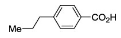
\includegraphics[width=0.25\columnwidth]{figs/q29a.png}
\captionof{figure}{Option A}
    \label{fig:q29a}
\item 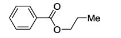
\includegraphics[width=0.25\columnwidth]{figs/q29b.png}
\captionof{figure}{Option B}
    \label{fig:q29b}
\item \includegraphics[width=0.25\columnwidth]{figs/q29c.png}
\captionof{figure}{Option C}
    \label{fig:q29c}
\item \includegraphics[width=0.25\columnwidth]{figs/q29d.png}
\captionof{figure}{Option D}
    \label{fig:q29d}
\end{enumerate}
\hfill (GATE CY 2020)

\item Major product formed in the following synthetic sequence is:

\begin{center}
\includegraphics[width=0.6\columnwidth]{figs/q30.png}
\captionof{figure}{Figure for Q.30}
 \label{fig:q30}
\end{center}

\begin{enumerate}
\item \includegraphics[width=0.35\columnwidth]{figs/q30a.png}
\captionof{figure}{Option A}
    \label{fig:q30a}
\item \includegraphics[width=0.35\columnwidth]{figs/q30b.png}
\captionof{figure}{Option B}
    \label{fig:q30b}
\item \includegraphics[width=0.35\columnwidth]{figs/q30c.png}
\captionof{figure}{Option C}
    \label{fig:q30c}
\item \includegraphics[width=0.35\columnwidth]{figs/q30d.png}
\captionof{figure}{Option D}
    \label{fig:q30d}
\end{enumerate}
\hfill (GATE CY 2020)

\item The \textbf{CORRECT} statement with respect to the stereochemistry of $\alpha$-hydroxy acids \textbf{P} and \textbf{Q} formed in the following reactions is:

\begin{center}
\includegraphics[width=0.6\columnwidth]{figs/q31.png}
\captionof{figure}{Figure for Q.31}
 \label{fig:q31}
\end{center}

\begin{enumerate}
\item Both P and Q are formed with retention of configuration.
\item Both P and Q are formed with inversion of configuration.
\item P is formed with retention of configuration and Q with inversion of configuration.
\item P is formed with inversion of configuration and Q with retention of configuration.
\end{enumerate}
\hfill (GATE CY 2020)

\item The rate of solvolysis of the given compounds is in the order:

\begin{center}
\includegraphics[width=0.6\columnwidth]{figs/q32.png}
\captionof{figure}{Figure for Q.32}
 \label{fig:q32}
\end{center}

\begin{enumerate}
\begin{multicols}{2}
\item T $>$ R $>$ O $>$ S $>$ P
\item O $>$ T $>$ R $>$ P $>$ S
\item R $>$ T $>$ O $>$ S $>$ P
\item T $>$ O $>$ T $>$ R $>$ S
\end{multicols}
\end{enumerate}
\hfill (GATE CY 2020)

\item In the following reaction sequence, the major products Q and R are:

\begin{center}
\includegraphics[width=0.6\columnwidth]{figs/q33.png}
\captionof{figure}{Figure for Q.33}
 \label{fig:q33}
\end{center}

\begin{enumerate}
\item \includegraphics[width=0.35\columnwidth]{figs/q33a.png}
\captionof{figure}{Option A}
    \label{fig:q33a}
\item \includegraphics[width=0.35\columnwidth]{figs/q33b.png}
\captionof{figure}{Option B}
    \label{fig:q33b}
\item \includegraphics[width=0.35\columnwidth]{figs/q33c.png}
\captionof{figure}{Option C}
    \label{fig:q33c}
\item \includegraphics[width=0.35\columnwidth]{figs/q33d.png}
\captionof{figure}{Option D}
    \label{fig:q33d}
\end{enumerate}
\hfill (GATE CY 2020)

\item In the electronic absorption spectrum of an aqueous solution of \(\mathrm{[Ni(NH_3)_6]^{2+}}\), a very weak band is observed between the bands due to the transitions \(^3A_{2g} \to {}^3T_{2g}\) and \(^3A_{2g} \to {}^3T_{1g}(F)\). The transition responsible for the very weak band is:

(Given: atomic number of Ni is 28)

\begin{enumerate}
\begin{multicols}{2}
\item \(^3A_{2g} \to {}^1T_{1g}\)
\item \(^3A_{2g} \to {}^1T_{2g}\)
\item \(^3A_{2g} \to {}^1E_{g}\)
\item \(^3A_{2g} \to {}^1A_{1g}\)
\end{multicols}
\end{enumerate}
\hfill (GATE CY 2020)

\item The experimental magnetic moment (3.4 BM) of a hydrated salt of \(\mathrm{Eu^{2+}}\) at 27 \(^\circ\mathrm{C}\) is significantly different from the calculated value. The difference is due to:

(Given: atomic number of Eu is 63)

\begin{enumerate}
\item population of electrons at higher \(J\) level(s) via thermal excitation.
\item strong ligand field splitting of \(f\)-orbitals.
\item strong spin–orbit coupling.
\item pairing of electrons in \(f\)-orbitals.
\end{enumerate}
\hfill (GATE CY 2020)

\item The \textbf{CORRECT} combination of L1 and L2 among \(\mathrm{H^-}\), \(\mathrm{NO^-}\), \(\mathrm{MeCH_2^-}\), \(\mathrm{MeCH^-}\), and CO, that will satisfy the 18-electron rule for both metal centers in the following neutral molecule, is:

\begin{center}
\includegraphics[width=0.5\columnwidth]{figs/q36.png}
\captionof{figure}{Figure for Q.36}
 \label{fig:q36}
\end{center}

(Given: atomic number of Ru is 44)

\begin{enumerate}
\begin{multicols}{2}
\item \(\mathrm{H^-}\), \(\mathrm{NO^-}\)
\item \(\mathrm{MeCH_2^-}\), \(\mathrm{NO^-}\)
\item \(\mathrm{MeCH_2^-}\), CO
\item \(\mathrm{H^-}\), CO
\end{multicols}
\end{enumerate}
\hfill (GATE CY 2020)

\item In the following reaction sequence,

\begin{center}
\includegraphics[width=0.6\columnwidth]{figs/q37.png}
\captionof{figure}{Figure for Q.37}
 \label{fig:q37}
\end{center}

the structure of B is

(Given: atomic number of Mo is 42)

\begin{enumerate}
\item \includegraphics[width=0.35\columnwidth]{figs/q37a.png}
\captionof{figure}{Option A}
    \label{fig:q37a}
\item \includegraphics[width=0.35\columnwidth]{figs/q37b.png}
\captionof{figure}{Option B}
    \label{fig:q37b}
\item \includegraphics[width=0.35\columnwidth]{figs/q37c.png}
\captionof{figure}{Option C}
    \label{fig:q37c}
\item \includegraphics[width=0.35\columnwidth]{figs/q37d.png}
\captionof{figure}{Option D}
    \label{fig:q37d}
\end{enumerate}
\hfill (GATE CY 2020)

\item The following table lists the reaction/conversion catalyzed by metalloenzymes.

\begin{center}
\begin{table}[htbp]
  \centering
  \caption{Table-3}
  \label{table3}
  \begin{tabular}{cc}
  \textbf{Processing Technique} & \textbf{Producct} \\ \\
    P. Calendering & 1. Pipes \\
    Q. Extrusion & 2. Disposable cups \\
    R. Injection moulding & 3. Sheets \\
    S. Thermoforming & 4. Nylon gears \\
  \end{tabular}
\end{table}
 \captionsetup{type=table}
\captionof{table}{Table for Q.38}
\end{center}

The CORRECT combination is

\begin{enumerate}
\begin{multicols}{2}
\item P-II; Q-I; R-III; S-IV
\item P-IV; Q-II; R-I; S-I
\item P-I; Q-II; R-IV; S-III
\item P-I; Q-IV; R-III; S-II
\end{multicols}
\end{enumerate}
\hfill (GATE CY 2020)

\item The fission reaction of $^{235}_{92}$U with thermal neutron is represented below.

\begin{center}
\includegraphics[width=0.7\columnwidth]{figs/q39.png}
\captionof{figure}{Figure for Q.39}
 \label{fig:q39}
\end{center}

$^{99}$Nb and $^{135}$Sb are the primary fission fragment pair, which undergo series of radioactive decay to form stable nuclei X$_3$ and Y$_4$ (chain enders). The X$_3$ and Y$_4$, respectively are:

\begin{enumerate}
\begin{multicols}{2}
\item $^{96}$Mo and $^{133}$Cs
\item $^{99}$Ru and $^{138}$Cs
\item $^{97}$Sr and $^{142}$Ba
\item $^{87}$Br and $^{143}$Ce
\end{multicols}
\end{enumerate}
\hfill (GATE CY 2020)

\item The CORRECT 'voltage (E) \emph{versus} time' excitation signal used in cyclic voltammetry is

\begin{enumerate}
\item \includegraphics[width=0.3\columnwidth]{figs/q40a.png}
\captionof{figure}{Option A}
    \label{fig:q40a}
\item \includegraphics[width=0.3\columnwidth]{figs/q40b.png}
\captionof{figure}{Option B}
    \label{fig:q40b}
\item \includegraphics[width=0.3\columnwidth]{figs/q40c.png}
\captionof{figure}{Option C}
    \label{fig:q40c}
\item \includegraphics[width=0.3\columnwidth]{figs/q40d.png}
\captionof{figure}{Option D}
    \label{fig:q40d}
\end{enumerate}
\hfill (GATE CY 2020)

\item The hydrogen-like radial wave function of the $3s$ orbital is given as

\[
R_{30} = \frac{1}{9 \sqrt{3}} \brak{\left(\frac{Z}{a_0}\right)^{3/2}} \brak{6 - 2\rho + \frac{\rho^2}{6}} e^{-\rho/6}
\]


where $\rho = 2Zr/a_0;~ Z$ = atomic number; $r$ = distance from the nucleus; and $a_0$ = Bohr radius.

Positions of the radial nodes (in units of $a_0$) of the $3s$ orbital are at

\begin{enumerate}
\item $\dfrac{3+\sqrt{3}}{2Z}, \dfrac{3-\sqrt{3}}{2Z}$
\item $\dfrac{6+3\sqrt{3}}{2Z}, \dfrac{6-3\sqrt{3}}{2Z}$
\item $\dfrac{9+3\sqrt{3}}{2Z}, \dfrac{9-3\sqrt{3}}{2Z}$
\item $\dfrac{3+3\sqrt{3}}{2Z}, \dfrac{3-3\sqrt{3}}{2Z}$
\end{enumerate}
\hfill (GATE CY 2020)

\item $\Delta G_f^\circ$ and $\Delta H_f^\circ$ for Fe(g) are $370.7~\text{kJ mol}^{-1}$ and $416.3~\text{kJ mol}^{-1}$ at 298 K, respectively. Assuming $\Delta H_f^\circ$ is constant in the interval 250 K to 375 K, $\Delta G_f^\circ$ (rounded off to the nearest integer) for Fe(g) at 375 K is:

\begin{enumerate}
\begin{multicols}{2}
\item 359 kJ mol$^{-1}$
\item 338 kJ mol$^{-1}$
\item 325 kJ mol$^{-1}$
\item 310 kJ mol$^{-1}$
\end{multicols}
\end{enumerate}
\hfill (GATE CY 2020)

\item Adsorption of N$_2$ on TiO$_2$ was carried out at 75 K. A plot of $\frac{z}{(1-z)p}$ versus $z$ ($z = p/p^0$) gives a straight line with an intercept, $4.0 \times 10^{-6}~\text{mm}^3$ and slope, $1.0 \times 10^{-3}~\text{mm}^3$. The volume (rounded off to the nearest integer) corresponding to the monolayer coverage is:

\begin{enumerate}
\begin{multicols}{2}
\item 996 mm$^3$
\item 785 mm$^3$
\item 690 mm$^3$
\item 555 mm$^3$
\end{multicols}
\end{enumerate}
\hfill (GATE CY 2020)

\item Among the following sets,

\begin{center}
\begin{figure}[H]
\includegraphics[width=0.6\columnwidth]{figs/q44.png}
\captionof{figure}{Figure for Q.44}
\end{figure}

\end{center}

the total number of set(s) of diastereomeric pair(s) is \underline{\hspace{2cm}}
\hfill (GATE CY 2020)

\item Among the following,

\begin{center}
\includegraphics[width=0.7\columnwidth]{figs/q45.png}
\captionof{figure}{Figure for Q.45}
\label{fig:q45}
\end{center}

the total number of compounds showing characteristic carbonyl stretching frequency less than 1700 cm$^{-1}$ in their IR spectra is \underline{\hspace{2cm}}
\hfill (GATE CY 2020)

\item Consider that AgX crystallizes in rock salt structure. The density of AgX is 6477 kg/m$^3$ and unit cell length is 577.5 pm. Atomic weight of Ag is 107.87 g mol$^{-1}$. The atomic weight of X (in g mol$^{-1}$, \textit{rounded off to two decimal places}) is \underline{\hspace{2cm}}
\hfill (GATE CY 2020)

\item The total number of $g_{11}$ lines expected in the EPR spectrum of a solution of bis(salicylaldimine) copper(II) having pure $^{63}$Cu and $^{14}$N at 77 K is \underline{\hspace{2cm}}

(Given: I values of $^{63}$Cu, $^{14}$N and $^1$H are $\frac{3}{2}$, 1 and $\frac{1}{2}$, respectively)
\hfill (GATE CY 2020)

\item Among the following,

[ \ce{[B2H12]^{2-}}, \ce{[NiS(CO)2]^{2-}}, \ce{[C2B5H11]^{2-}}, \ce{Rh3(CO)16}, \ce{Os6(CO)20}, \ce{B5H11}, \ce{B6H10} ]

the total number of species having \textit{nido} structure is \underline{\hspace{2cm}}

(Given: atomic numbers of H, B, C, O, Ni, Rh and Os are 1, 5, 6, 8, 28, 45 and 76, respectively)
\hfill (GATE CY 2020)

\item The frequency (in cm$^{-1}$, \textit{rounded off to two decimal places}) for pure rotational line in the spectrum of NO molecule due to change in the quantum number from $J=1$ to $J=2$ is \underline{\hspace{2cm}}

(Given: Moment of inertia of NO = $1.6427 \times 10^{-46}$ kg m$^{2}$; $h = 6.626 \times 10^{-34}$ J s; $c = 3 \times 10^8$ m/s)
\hfill (GATE CY 2020)

\item The \% error (\textit{rounded off to two decimal places}) in the ground state energy of a particle in a one dimensional box of length `a' described by a trial variation function $\varphi = x(a-x)$, where $0 \leq x \leq a$, is \underline{\hspace{2cm}}

(Given: The true ground state energy of the above system is $h^2/(8ma^2)$; $\int_{0}^{a} \varphi^2 dx = a^5/30$)
\hfill (GATE CY 2020)

\item Assuming no interaction between vibrational and rotational energy levels in HF, the frequency (in cm$^{-1}$, \textit{rounded off to the nearest integer}) of the R branch line originating from $J=4$ in its IR spectrum is \underline{\hspace{2cm}}

(Given: Rotational constant for HF = 19.35 cm$^{-1}$; $\tilde{\nu}_0 = 4138.52$ cm$^{-1}$)
\hfill (GATE CY 2020)

\item The van der Waals constants $a$ and $b$ for gaseous CO are given as $1.49~\text{L}^2~\text{atm mol}^{-2}$ and $0.0399~\text{L mol}^{-1}$, respectively. The fugacity (in atm, \textit{rounded off to two decimal places}) of CO at 35$^\circ$C and 95 atm is \underline{\hspace{2cm}}

(Given: $R = 0.082~\text{L atm K}^{-1}~\text{mol}^{-1}$)
\hfill (GATE CY 2020)

\item At 30$^\circ$C, the vapor pressure and density of a 1.0 M aqueous solution of sucrose are 31.207 mm Hg and 1.1256 g/mL, respectively. If the vapor pressure of pure water at 30$^\circ$C is 31.824 mm Hg, the activity coefficient (\textit{rounded off to three decimal places}) of water in the given solution is \underline{\hspace{2cm}}

(Given: The molar mass of sucrose = $342.3~\text{g mol}^{-1}$)
\hfill (GATE CY 2020)

\item For the ring opening reaction of cyclopropane to propene at 25$^\circ$C, the pre-exponential factor is $4.3 \times 10^{15}~\text{s}^{-1}$. The entropy of activation (in J K$^{-1}$ mol$^{-1}$, \textit{rounded off to two decimal places}) is \underline{\hspace{2cm}}

(Given: $h = 6.626 \times 10^{-34}$ Js; $k_B = 1.38 \times 10^{-23}$ K$^{-1}$; $R = 8.314$ J K$^{-1}$ mol$^{-1}$)
\hfill (GATE CY 2020)

\item In a reaction, reactant X is converted to products Y and Z consecutively with rate constants $6.0 \times 10^{-2}$ min$^{-1}$ and $9.0 \times 10^{-3}$ min$^{-1}$, respectively. If the initial amount of X is 12.5 moles, the number of moles (\textit{rounded off to one decimal place}) of Y formed after 10 minutes is \underline{\hspace{2cm}}
\hfill (GATE CY 2020)



\end{enumerate}
\end{document}
